\documentclass[12pt]{article}
\usepackage[left=1cm, right=1cm, top=2cm,bottom=1.5cm]{geometry} 

\usepackage[parfill]{parskip}
\usepackage[utf8]{inputenc}
\usepackage[T2A]{fontenc}
\usepackage[russian]{babel}
\usepackage{enumitem}
\usepackage[normalem]{ulem}
\usepackage{amsfonts, amsmath, amsthm, amssymb, mathtools}

\usepackage{fancyhdr}
\pagestyle{fancy}
\renewcommand{\headrulewidth}{1.5pt}
\renewcommand{\footrulewidth}{1pt}

\usepackage{graphicx}
\usepackage[figurename=Рис.]{caption}
\usepackage{subcaption}
\usepackage{float}

%%Наименование папки откуда забирать изображения
\graphicspath{ {./images/} }

%%Изменение формата для ввода доказательства
\renewcommand{\proofname}{$\square$  \nopunct}
\renewcommand\qedsymbol{$\blacksquare$}

\addto\captionsrussian{%
	\renewcommand{\proofname}{$\square$ \nopunct}%
}
%% Римские цифры
\newcommand{\RN}[1]{%
	\textup{\uppercase\expandafter{\romannumeral#1}}%
}


\theoremstyle{definition}
\newtheorem{defn}{Опр:}
\newtheorem{rem}{Rm:}
\newtheorem{prop}{Утв.}
\newtheorem{exrc}{Упр.}
\newtheorem{lemma}{Лемма}
\newtheorem{theorem}{Теорема}
\newtheorem{corollary}{Следствие}

\newenvironment{cusdefn}[1]
{\renewcommand\thedefn{#1}\defn}
{\enddefn}



\DeclareRobustCommand{\divby}{%
	\mathrel{\text{\vbox{\baselineskip.65ex\lineskiplimit0pt\hbox{.}\hbox{.}\hbox{.}}}}%
}


\newcommand{\smallerrel}[1]{\mathrel{\mathpalette\smallerrelaux{#1}}}
\newcommand{\smallerrelaux}[2]{\raisebox{.1ex}{\scalebox{.75}{$#1#2$}}}

\newcommand{\smallin}{\smallerrel{\in}}
\newcommand{\smallnotin}{\smallerrel{\notin}}

\newcommand*{\medcap}{\mathbin{\scalebox{1.25}{\ensuremath{\cap}}}}%
\newcommand*{\medcup}{\mathbin{\scalebox{1.25}{\ensuremath{\cup}}}}%

\begin{document}
\lhead{Математический анализ - I}
\chead{Шапошников С.В.}
\rhead{Лекция - 13}
	
\begin{theorem}\textbf{Бэра}:
	Пусть $F$ - не пустое, замкнутое подмножество $\mathbb{R}$ и $F = \bigcup\limits_{n} F_n$ - не более, чем счетное объединение замкнутых множеств $F_n$, тогда $\exists \, N$ и $(\alpha, \beta) \colon F \cap (\alpha,\beta) \neq \varnothing \wedge F \cap (\alpha,\beta) \subset F_N$. 
	
	В частности, если $\mathbb{R} = \bigcup\limits_n F_n$, то хотя бы одно из $F_n$ содержит интервал.
\end{theorem}

\textbf{Пример}: $[a,b], \, a < b$ - не является счетным. 
\begin{proof}
	\uline{От противного}: пусть он является счетным $\Rightarrow [a,b] =  \bigcup\limits_n \{x_n\}$, точка - замкнута $\Rightarrow$ получили счетное объединение замкнутых множеств. По теореме $\exists \, (\alpha, \beta) \colon [a,b] \cap (\alpha,\beta) \neq \varnothing \wedge [a,b] \cap (\alpha, \beta) \subset \{x_n\}$, но пересечение интервала с отрезком - всегда не одноточечное множество.
\end{proof}

\textbf{Пример}: С помощью теоремы Бэра также можно показать, что $\mathbb{R}$ - не является счетным.

\textbf{Пример}: Множество иррациональных чисел нельзя представить в виде не более, чем счетного набора замкнутых множеств. Иначе, множество рациональных чисел - счетно, множество иррациональных чисел - счетно $\Rightarrow \mathbb{R}$ - объединение счетного набора замкнутых множеств (точки - замкнуты).

\begin{proof}\textbf{Доказательство теоремы Бэра}\\
	\uline{От противного}: Ни для какого $N$ не найдется требуемого интервала $(\alpha, \beta)$.
	
	\uline{$\RN{1}$-ый шаг}:
	
	Возьмем $F \cap (\mathbb{R} \setminus F_1) \neq \varnothing$, иначе $F = F_1 \Rightarrow a \in F \Rightarrow (a-\varepsilon, a + \varepsilon) \cap F \subset F_1$.
	
	\begin{figure}[H]
		\centering
		\includegraphics[width=0.35\textwidth]{13_1.eps}
		\caption{Точка $a_1 \in F \cap (\mathbb{R} \setminus F_1)$.}
		\label{13_1}
	\end{figure}
	
	Возьмем точку $a_1 \in F \cap (\mathbb{R} \setminus F_1)$, тогда $\exists \, (\alpha_1,\beta_1) \colon a_1 \in (\alpha_1,\beta_1) \wedge (\alpha_1,\beta_1) \subset (\mathbb{R}\setminus F_1)$. Более того, можно взять отрезок $[\alpha_1,\beta_1]$ внутри заданного интервала: ужать интервал, взять отрезок и переименовать его, как $[\alpha_1,\beta_1]$:
	
	\begin{figure}[H]
		\centering
		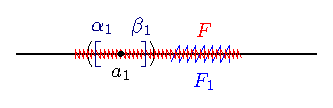
\includegraphics[width=0.35\textwidth]{13_2.eps}
		\caption{Ужатие интервала до отрезка.}
		\label{13_2}
	\end{figure}
	
	Можно его ужать так, что $\beta_1 - \alpha_1 < 1$. Итог $\RN{1}$-го шага - построен отрезок $[\alpha_1,\beta_1]$:
	\begin{enumerate}[label={\arabic*)}]
		\item $\beta_1 - \alpha_1 < 1$;
		\item $(\alpha_1, \beta_1) \cap F \neq \varnothing$ (там точно есть $a_1$);
		\item $[\alpha_1, \beta_1] \subset \mathbb{R} \setminus F_1$ (значит у этого отрезка нет точек из $F_1$);
	\end{enumerate}

	\uline{$\RN{2}$-ый шаг}:
	
	Посмотрим на интервал: $(\alpha_1, \beta_1) \cap F \neq \varnothing \Rightarrow (\alpha_1, \beta_1) \cap F \not\subset F_2$, иначе предположение от противного было бы не верно и требуемое $N = 2$. 
	Тогда $\exists \, a_2 \in (\alpha_1,\beta_1) \cap F \wedge a_2 \notin F_2$. 
	
	\begin{figure}[H]
		\centering
		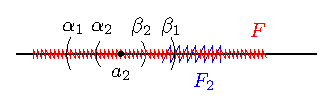
\includegraphics[width=0.35\textwidth]{13_3.eps}
		\caption{Построение второго интервала на $\RN{2}$-ом шаге.}
		\label{13_3}
	\end{figure}
	
	Дополнение к $F_2$ - открытое множество $\Rightarrow a_2$ в него входит с некоторым интервалом ($(\alpha_1, \beta_1)$ не обязательно полностью лежит в $F$) $\Rightarrow$ аналогично $\RN{1}$-му шагу, $\exists$ интервал $(\alpha_2, \beta_2)$:
	\begin{enumerate}[label={\arabic*)}]
		\item $\beta_2 - \alpha_2 < \dfrac{1}{2}$;
		\item $(\alpha_2, \beta_2) \cap F \neq \varnothing$ (там точно есть $a_2$);
		\item $[\alpha_2, \beta_2] \subset \mathbb{R} \setminus F_2$ (значит у этого отрезка нет точек из $F_2$);
		\item $[\alpha_2,\beta_2] \subset [\alpha_1, \beta_1]$;
	\end{enumerate}

	\uline{$\RN{3}$-ий шаг}:
	
	Рассмотрим интервал: $(\alpha_2, \beta_2) \cap F \neq \varnothing \Rightarrow (\alpha_2, \beta_2) \cap F \not\subset F_3$, иначе предположение от противного было бы не верно и требуемое $N = 3$. 
	Тогда $\exists \, a_3 \in (\alpha_2,\beta_2) \cap F \wedge a_3 \notin F_3$. 
	
	\begin{figure}[H]
		\centering
		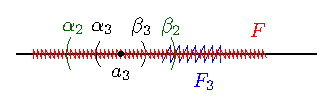
\includegraphics[width=0.35\textwidth]{13_4.eps}
		\caption{Построение второго интервала на $\RN{3}$-ем шаге.}
		\label{13_4}
	\end{figure}
	
	Дополнение к $F_3$ - открытое множество $\Rightarrow a_3$ в него входит с некоторым интервалом ($(\alpha_2, \beta_2)$ не обязательно полностью лежит в $F$) $\Rightarrow$ аналогично $\RN{2}$-му шагу, $\exists$ интервал $(\alpha_3, \beta_3)$:
	\begin{enumerate}[label={\arabic*)}]
		\item $\beta_3 - \alpha_3 < \dfrac{1}{3}$;
		\item $(\alpha_3, \beta_3) \cap F \neq \varnothing$ (там точно есть $a_3$);
		\item $[\alpha_3, \beta_3] \subset \mathbb{R} \setminus F_3$ (значит у этого отрезка нет точек из $F_3$);
		\item $[\alpha_3,\beta_3] \subset [\alpha_2,\beta_2] \subset [\alpha_1, \beta_1]$;
	\end{enumerate}
	
	И так далее, пока не получим систему вложенных отрезков $[\alpha_1,\beta_1] \supset [\alpha_2,\beta_2] \supset \dotsc$ таких, что \\
	$[\alpha_n, \beta_n] \cap F \neq \varnothing, \, \beta_n - \alpha_n < \dfrac{1}{n}$ и $[\alpha_n, \beta_n] \cap F_n = \varnothing$. По теореме о вложенных отрезках $\exists \, c \in \bigcap\limits_{n}[\alpha_n,\beta_n]$. Очевидно, что $c \notin F_n, \, \forall n$ по построению. Если $c \notin F \Rightarrow c \in \mathbb{R} \setminus F \Rightarrow \exists \, (\alpha,\beta) \colon c \in (\alpha, \beta) \wedge (\alpha,\beta) \cap F = \varnothing$.

	\begin{figure}[H]
		\centering
		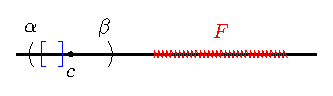
\includegraphics[width=0.35\textwidth]{13_5.eps}
		\caption{Точка $c$, принадлежащая пересечению всех вложенных отрезков.}
		\label{13_5}
	\end{figure}

	Отрезки стягиваются к точке $c$: как только $\beta_n - \alpha_n < \min \{\beta-c,c-\alpha\}$, то этот отрезок целиком будет лежать в $(\alpha,\beta)$, то есть $[\alpha_n, \beta_n] \subset (\alpha, \beta)$, что невозможно, так как в $(\alpha, \beta)$ нет точек из $F$. \\
	Тогда $c \in F = \bigcup\limits_{n} F_n \wedge c \notin F_n, \, \forall n \Rightarrow$ противоречие.
\end{proof}

\section*{Компакты}

\begin{defn}
	Множество $K \subset \mathbb{R}$ называется \uwave{компактом}, если для всякого набора открытых множеств $\{\mathcal{U}_\alpha\}$ такого, что $K \subset \bigcup\limits_{\alpha}\mathcal{U}_\alpha$, найдется конечный поднабор $\mathcal{U}_{\alpha_1}, \dotsc, \mathcal{U}_{\alpha_N} \colon K \subset \bigcup\limits_{k=1}^N \mathcal{U}_{\alpha_k}$. То есть, из всякого покрытия $K$ открытыми множествами можно выбрать конечное подпокрытие.
\end{defn}

\textbf{Пример (не компакт)}: рассмотрим интервал $(0,1)$ и возьмем другой интервал $(\frac{1}{n},1)$ очевидно, что $(0,1) = \bigcup\limits_n (\frac{1}{n},1) \Rightarrow$ нет конечного набора, который покрыл бы $(0,1) \Rightarrow$ не компакт.

\begin{figure}[H]
	\centering
	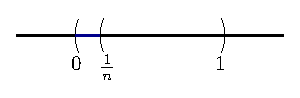
\includegraphics[width=0.3\textwidth]{13_6.eps}
	\caption{Пример не компакта.}
	\label{13_6}
\end{figure}

\textbf{Пример (компакт)}:  точка является компактом. $a \in \bigcup\limits_{\alpha}\mathcal{U}_\alpha \Leftrightarrow \exists \, \mathcal{U}_\alpha \colon a \in \mathcal{U}_\alpha$.

\begin{figure}[H]
	\centering
	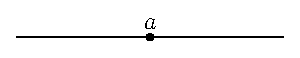
\includegraphics[width=0.27\textwidth]{13_7.eps}
	\caption{Точка $a$ - пример компакта.}
	\label{13_7}
\end{figure}

\begin{lemma}\textbf{(Бореля-Гейне-Лебега)}:
	Отрезок - это компакт.
\end{lemma}
\begin{proof}
	\uline{От противного}: Пусть у отрезка $[a,b], \, a < b, \, \exists$ покрытие $\{\mathcal{U}_\alpha\}$ из которого нельзя выбрать конечное подпокрытие. Делим отрезок $[a,b]$ пополам и выбираем в качестве отрезка $[a_1,b_1]$ ту половину у которой нет конечного подпокрытия в покрытии $\{\mathcal{U}_\alpha\}$. \\
	Такая половина есть, так как иначе у исходного отрезка было бы конечное подпокрытие.
	
	Повторяем то же самое с $[a_1,b_1]$: делим $[a_1,b_1]$ пополам и выбираем в качестве отрезка $[a_2,b_2]$ ту половину у которой нет конечного подпокрытия в покрытии $\{\mathcal{U}_\alpha\}$. 
	
	И так далее, по аналогии получаем систему вложенных отрезков, которые нельзя покрыть конечным набором подпокрытий:
	$$[a_1,b_1] \supset [a_2,b_2] \supset \dotsc \supset [a_n, b_n] \supset \dotsc$$ 
	причем $b_n - a_n = \frac{b-a}{2^n} \to 0$ (длины стремятся к нулю). 
	
	По теореме о вложенных отрезках $\exists \, c \colon c \in \bigcap\limits_n [a_n,b_n]$. Кроме того, $c \in [a,b] \subset \bigcup\limits_{\alpha}\mathcal{U}_\alpha \Rightarrow \exists \, \alpha \colon c \in \mathcal{U}_\alpha$. Так как $\mathcal{U}_\alpha$ - открыто, то $\exists$ интервал $\mathcal{U}(c) = (s,t) \subset \mathcal{U}_\alpha$. В этом случае $$\exists \, n \colon b_n - a_n < \min \{c-s, t-c\} \Rightarrow [a_n,b_n] \subset \mathcal{U}(c) \subset \mathcal{U}_\alpha$$
	
	То есть отрезок $[a_n, b_n]$ покрыт одним множеством $\mathcal{U}_\alpha$ - это противоречит построению.
\end{proof}

\subsection*{Свойства компактов}
\begin{enumerate}[label={(\arabic*)}]
	\item Компакт - ограниченное множество, то есть лежит в некотором отрезке;
	\begin{proof}
		\begin{figure}[H]
			\centering
			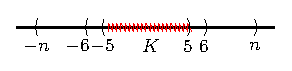
\includegraphics[width=0.27\textwidth]{13_8.eps}
			\caption{Ограниченность компакта.}
			\label{13_8}
		\end{figure}
		Пусть $K$ - компакт, тогда $K \subset \bigcup\limits_n(-n,n)$ (потому, что там лежит все $\mathbb{R}$). Но по определению компакта $\exists \, n_1, \dotsc, n_N \colon K \subset \bigcup\limits_{s=1}^N(-n_s,n_s)$. Предположим, что $C = \max\limits_{1 \leq s \leq N} n_s$, тогда $K \subset (-C, C)$.
	\end{proof}
	\item Компат - замкнутое множество;
	\begin{proof}
		Необходимо доказать, что дополнение к этому множеству - открыто. Пусть $K$ - компакт, возьмем $a \in \mathbb{R} \setminus K$. 
		
		Как доказать, что дополнение открыто? Надо доказать, что всякая такая точка $a$ входит в дополнение с некоторым интервалом. Возьмем отрезок $[a -\frac{1}{n}, a + \frac{1}{n}]$
		
		\begin{figure}[H]
			\centering
			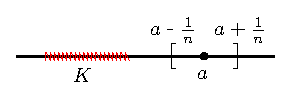
\includegraphics[width=0.27\textwidth]{13_9.eps}
			\caption{Точка из дополнения компакта в отрезке: $a \in \mathbb{R} \setminus K$.}
			\label{13_9}
		\end{figure}
		 и будем брать дополнение к этому отрезку: $\mathcal{U}_n = \mathbb{R}\setminus [a -\frac{1}{n}, a + \frac{1}{n}]$. 
		
		\begin{figure}[H]
			\centering
			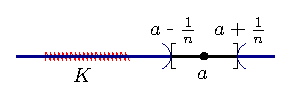
\includegraphics[width=0.27\textwidth]{13_10.eps}
			\caption{Стягивание множества $\mathcal{U}_n$ к точке $a$.}
			\label{13_10}
		\end{figure}
		
		Если взять объединение всех таких множеств, то получим всю прямую без точки $a$: $\bigcup\limits_n \mathcal{U}_n = \mathbb{R} \setminus \{a\}$. Но это содержит компакт $K \colon K \subset \mathbb{R} \setminus \{a\} \Rightarrow$ объединение лучей (откр. множеств) содержит $K$.
		
		По определению $\exists$ конечное подпокрытие $\mathcal{U}_{n_1}, \dotsc ,\mathcal{U}_{n_N} \Rightarrow$ возьмем $M = \max\limits_{1\leq s \leq N} \{n_s\}$.\\
		Тогда $\mathbb{R}\setminus [a - \frac{1}{M}, a+ \frac{1}{M}] \supset K \Rightarrow$ взяли из этого набора лучей тот, который наиболее близко подошел к точке $a \Rightarrow (a - \frac{1}{M}, a+ \frac{1}{M}) \subset \mathbb{R} \setminus K$, то есть $\mathbb{R} \setminus K$ - открыто.		
	\end{proof}
	\item Если замкнутое множество $F$ является подмножеством компакта $K$, то $F$ - компакт;
	\begin{proof}
		Пусть $F \subset \bigcup\limits_\alpha \mathcal{U}_\alpha \Rightarrow K \subset \bigcup\limits_\alpha \mathcal{U}_\alpha \cup (\mathbb{R} \setminus F)$. По определению существует конечное подпокрытие: $\mathcal{U}_{\alpha_1}, \dotsc, \mathcal{U}_{\alpha_N}$ и может быть $(\mathbb{R} \setminus F)$ 	- они будут покрывать $K \Rightarrow$ 
		
		$$F \subset \mathcal{U}_{\alpha_1} \cup \dotsc \cup \mathcal{U}_{\alpha_N} \cup (\mathbb{R} \setminus F) = \mathcal{U}_{\alpha_1} \cup \dotsc \cup \mathcal{U}_{\alpha_N}$$ 
		
		$\Rightarrow$ у $F$ есть конечное подпокрытие.
	\end{proof}
\end{enumerate}

\begin{corollary}\textbf{(Критерий компактности)}:
	$K \subset \mathbb{R}$ - компакт $\Leftrightarrow K$ - ограничено и замкнуто.
\end{corollary}

\begin{proof}\hfill\\
	$(\Rightarrow)$ очевидно по свойствам компакта.
	
	$(\Leftarrow)$ $K$ - ограниченно $\Rightarrow \exists \, [a,b] \colon K \subset [a,b]$. Отрезок $[a,b]$ - компакт, $K$ - замкнуто, тогда по свойству $(3) \Rightarrow K$ - компакт.
\end{proof}

\end{document}